\chapter{Implementation of AXL\label{chap:imp}}

The AXL compiler translates AXL programs into C++ code. For instance,
the classifier algorithm of Example \ref{exe:sprint}, compiles into
more than 2100 lines of C++ code. AXL adopts an open interface for its
physical data model, so that the system can link with a variety of
physical database implementations.  Currently, we use the Berkeley DB
library\cite{berkeley} as our main storage manager.

% Aggregates in AXL are hash-based by default. However, we
% also allow the use of predicates like {\cdf SORT BY column} or {\cdf
%   SORT BY GROUPBY} in a UDA to force sort-based aggregation.

The runtime model of AXL is based on data pipelining. In particular,
all UDAs, including recursive UDAs that call themselves, are
pipelined; thus, tuples inserted into the RETURN relation during the
INITIALIZE/ITERATE steps are returned to their caller immediately.
Therefore, local variables (temporary tables) declared in a UDA can
not reside on the stack. They are assembled into a {\tt state}
structure which is then passed to the UDA for each
INITIALIZE/ITERATE/TERMINATE call, so that these internal data are not
lost between the calls.

The current AXL implementation has more than 33,000 lines of C++ code.
We are working on to add more SQL data types, O-R database extensions
and a richer set of supporting indexes and storage structures. We
expect the complete and more robust system will eventually have 90,000
lines of code.


\section{AXL Query Graph}
The AXL system is composed of three major modules: the parser, the
rewriter and the code generator.

The core data structure in AXL is the query graph, which is used by
all AXL modules. The parser builds initial query graphs based on the
abstract syntax tree. The rewriter makes changes to the query graphs.
Finally, the code generator translates the query graphs into C++ code.

A query graph is composed of a set of nodes and arcs. A node
represents some kind of operation, for instance, SELECT, INSERT and
DELETE. Some operations can be pipelined (SELECT statement without the
DISTINCT flag), others are blocking (ORDER, GROUP-BY, and etc.). An
arc connecting a parent node and a child node represents the fact that
the parent node consumes the data stream produced by the child node.

\section{The AXL Parser}

For each SQL statement, the parser builds a primitive query graph,
which is essentially the abstract syntax tree.

\subsubsection*{Node Data Structure} 
A node in the query graph is represented by the following data
structure:
\begin{itemize}
\item {\it Type of the node.} The types are described below.
\item {\it Flags.} The most important flag used is the DISTINCT flag,
  indicating whether duplicate tuples are allowed in the data stream
  produced by the current node.
\item {\it A list of {\tt (exp, alias)} pairs.} This list describes
  the tuple in the output stream. Each column of the tuple can be
  referenced by its alias.
\item {\it A list of predicates.}  For a SELECT node, the WHERE
  clause, as well as the HAVING clause, is decomposed into
  conjunctions of predicates.  All the tuples produced by a SELECT
  node must satisfy its own predicates. 
\item {\it A list of arcs connecting the current node to its child
    nodes.}  Tuples are passed by the child nodes along the arcs to
  their parent node. The structure of the data passed along the arc
  is describe by the list of {\tt (exp, alias)} pairs in the child
  node.
\end{itemize}

\subsubsection*{Node Types} 

A node in the query graph can have any of the following types:
\begin{itemize}
\item A\_SQL\_SEL\\
  SQL SELECT statements are represented by SELECT nodes in a query
  graph.
  
  The initial abstract syntax tree built by the parser for a SELECT
  statement is different from the SELECT node in a query graph. The
  abstract syntax tree for a SELECT statement may contain aggregates,
  a GROUP-BY clause, a HAVING condition, and even an ORDER-BY clause.
  These, however, are represented and implemented by the GB node and
  the ORDER-BY node in a query graph.
  
  The rewriting of SELECT statements containing aggregates, GROUP-BY
  clauses, HAVING conditions, and ORDER-BY clauses is discussed in
  detail in Section \ref{sec:selstack}. The only trivial rewriting
  taken place during parsing is for the builtin aggregate {\tt avg}.
  An {\tt avg(x)} expression is rewritten into {\tt sum(x)/count(x)}
  when the abstract syntax tree is constructed.
  
\item A\_SQL\_GB\\
  Group-by and aggregates are represented by a GB node. A GB node has
  only one input stream. We overload the predicate list in the node
  structure to represent the GROUP-BY columns.
  
  GB node is not constructed by the parser, but instead, by the
  rewriter (Section \ref{sec:selstack}).
\item A\_SQL\_UNION\\
  A UNION node can have multiple child nodes. It combines the input
  stream coming from the child nodes to produce its own output stream.
  If the DISTINCT flag is set, then the UNION node should eliminate
  duplicate tuples. 
\item A\_SQL\_EXCEPT\\
  An EXCEPT node has two child nodes. It is not yet implemented in the
  current version of AXL.
\item A\_SQL\_INTERSECT\\
  An INTERSECT node has two child nodes. It is not yet implemented in
  the current version of AXL.
\item A\_SQL\_INSERT\\
  An INSERT node has two child nodes. It takes tuples from the left
  stream and insert them into the right child node. Since INSERT node
  does not have any output stream, it is usually the top most-node in
  a query graph.
\item A\_SQL\_DELETE\\
  A DELETE node has only one child node. As in the case of the INSERT
  node, the DELETE node does not have any output stream; it is usually
  the top-most node in a query graph.
\item A\_SQL\_UPDATE\\
  An UPDATE node has only one child node. As in the case of the INSERT
  and the DELETE node, the UPDATE node does not have any output
  stream; it is usually the top-most node in a query graph.
\item A\_SQL\_LOAD \\
  We use the LOAD node to bulk load data in text format from file
  systems into the AXL database system.
\item A\_SQL\_ORDER \\
  An ORDER node orders tuples from its incoming stream. We overload
  the predicate list in the node structure to represent the ORDER-BY
  columns.
\end{itemize}

\subsubsection*{Arc Types}
An arc in a query graph represents an incoming stream. There are
three different types of arcs. 

\begin{itemize}
\item {\it Source table.} The input stream comes from a source
  relation declared in the AXL problem.
\item {\it Table function.} A table function is an external function
  that returns a stream instead of a scalar value. Table functions can
  be used to enable the user to make almost any source of data appear
  to be an AXL table.
\item {\it Subquery.} A subquery is just a sub AXL graph. The input
  stream comes from the top node of the subgraph.
\end{itemize}

\section{The AXL Rewriter}
After initial query graphs are built during parsing, the rewriter will
make changes to the query graphs. A query graph is often expanded or
condensed according to the rewriting criteria. The rewriter is a very
important module, since much optimization is carried out during this
step.

The function {\tt rewriteQuery()} is the main routine that carries out
the necessary SQL rewriting. Currently, only three rewriting
operations are implemented: i) rewriting the SQL SELECT statements
that contain aggregates and/or the GROUP-BY clause, ii) rewriting the
SQL SELECT statements that contain the ORDER-BY clause, and iii)
expanding head expressions that return complex data types in a SELECT
box. A lot of useful rewritings can be added in the future to the {\tt
  rewriteQuery()} function. For instance, an important rewriting task
left for the new version of AXL is predicate push-up and push-down.


\subsection{Rewriting SELECT Statements for Aggregation\label{sec:selstack}}

Group-by and aggregation is a much more complex operation than a
simple SELECT operation which handles only select-project-join
operations. The abstract syntax tree for statements that contain
group-by and aggregates can be very complicated.  In AXL, therefore,
we decompose these SELECT statements by using SELECT nodes and GB
nodes.

In AXL, a SELECT statement using aggregation (with or without group-by
columns) is represented by three nodes one on top of another in the
query graph (Figure \ref{fig:stack}).

{\footnotesize
\begin{codedisplay}
\>\kw{SELECT} g$_1$, ..., g$_m$, aggr-exp$_1$, ..., aggr-exp$_n$\\
\>\kw{FROM} t$_1$, ..., t$_i$\\
\>\kw{WHERE} p$_1$ \kw{AND} ... \kw{AND} p$_j$\\
\>\kw{GROUP BY} g$_1$, ...,  g$_k$\\
\>\kw{HAVING} h$_1$ \kw{AND} ... \kw{AND} h$_l$
\end{codedisplay}
}

\begin{figure}[!htb]
\centering
\includegraphics[height=6cm]{stack.eps}
\caption{Rewriting SELECT Statements Using 3 Nodes}
\label{fig:stack}
\end{figure}
  
In Figure \ref{fig:stack}, the above SELECT statement is represented
by three query graph nodes. The GB node between the two SELECT nodes
is responsible for aggregation. It is clear that a GB node always has
one child node. Note that the expressions in the predicate list for
the GB node are actually the group by columns, and each group by
column is in its simplest form, i.e., either it is a constant or a
variable. The initial GROUP BY column that contains a complex
expression, for example, {\tt x+y}, can always be renamed to a new
variable {\tt a} in the SELECT node beneath the GB node by adding an
extra ``{\tt x+y AS a}'' expression in its SELECT list. This greatly
simplifies the optimization and code generation process for
aggregates.

\subsection{Rewriting SELECT Statement for Ordering}
A SELECT statement that contains an ``ORDER BY'' clause is represented
by two nodes in the query graph: an ORDER node and a SELECT node.
After getting tuples from the SELECT node beneath it, the ORDER node
stores the tuples in a buffer (or external file), sorts the buffer,
and then returns the tuples in a certain order.

\subsection{Expanding Complex Data Structure}
In AXL, a UDA can return a complex data type which consists of several
basic types. Suppose that the UDA {\tt aggr()} is defined as:

\begin{codedisplay}
AGGREGATE aggr(...): (INT a, CHAR b(20))
\end{codedisplay}

Then, the following SELECT statement (alias {\tt AS (c, d)} is
optional)

\begin{codedisplay}
\kw{SELECT} ..., aggr(...) \kw{AS} (c, d) , ...
\end{codedisplay}

is expanded into:

\begin{codedisplay}
\kw{SELECT} ..., aggr(...) $\rightarrow$ a \kw{AS} c, aggr(...) $\rightarrow$ b \kw{AS} d , ...
\end{codedisplay}


\section{The AXL Code Generator}
The code generator is responsible for type checks and C++ code
generation. Function {\tt trans2C()} is the entry routine to translate
a query graph to C++ code.

\subsection{Overview of Code Generation\label{sec:cgoverview}}

\subsubsection*{Evaluation of the Query Graph}
Figure \ref{fig:evalqg} shows a typical query graph for a SELECT node.
AXL uses pipelining as much as possible. We describe here how we get a
tuple from node A.

\begin{figure}[!htb]
\centering
\includegraphics[height=6cm]{evalqg.eps}
\caption{Evaluation of Query Graph}
\label{fig:evalqg}
\end{figure}

To get the next tuple from a node, we ask its current child node. For
each node, we keep a variable $index$ ($0 \le index < $\# of its child
nodes). The value of $index$ in the parent node indicates from which
child node we are currently getting the next tuple.  When we
successfully get a tuple from one child node, we increase $index$ of
the parent node by 1. So next time, we will get a tuple from the right
sibling of the current child node. If the current node is the right
most child node, then we successfully get a tuple from the parent
node. If the current child node fails to return a tuple, we backtrack
by decreasing $index$, so next time, we will try to get a tuple from
its left sibling node. If $index=0$, which means we are already
looking at the left most child node, then the parent node can not
produce any more tuples.

This is only a general picture of query graph evaluation procedure.
Things are more complicated in reality. For instance, we need to take
advantage of indexes available in source tables when we are trying to
get tuples from the child nodes. Also, if a node is blocking (for
instance, a group-by node or a sort node), we might need to store all
the tuples temporarily before we can return any of them to its parent
node.

\subsubsection*{Declaration, Execution and Clean-Up}
To generate C++ code for an AXL object (e.g., an SQL statement, an
expression, or a subquery), we call {\tt transExp(obj)} (or {\tt
  transDec(obj)} and etc., depending on the type of the object).
Usually three pieces of code are generated for the object: i) the
declaration code, ii) the execution code, and iii) the code for
clean-up.  It is responsibilities of the function caller to assemble
these three pieces of code.

For instance, when we generate code for an expression which contains
declarations of local tables, we need to generate C++ code to declare
AXL database handlers (as of now, the Berkeley DB database handlers).
Then, before the code for any SQL statement can be executed, we need
to call Berkeley DB APIs to open the tables that are used in the SQL
statement. Finally, when the SQL statement is done, we need to close
the Berkeley DB tables, and this piece of code is called the clean-up
code.

\subsubsection*{AXL Object ID}
Before we discuss the details of the code generation, we need to know
how to identify an AXL object. All components of the query graph,
including nodes, arcs, expressions and SQL statements, are AXL
objects.  An AXL object can be referenced by its identifiers, as
follows:

\begin{itemize}
\item {\it Static identifier.} Each AXL object in the query graph is
  uniquely identified by its static identifier.
\item {\it Dynamic identifier.} When the code generated from the query
  graph is being executed, in addition to the static identifier, an
  AXL object can have a dynamic identifier as well. For instance, an
  aggregate in a SELECT statement has a static identifier.  Every time
  it is invoked, it is assigned a unique dynamic identifier.  Thus, we
  differentiate calls to the same aggregate function at different
  levels of recursion.
\end{itemize}

\subsubsection*{Storage Manager}
Currently, Berkeley DB library is used as AXL's main storage manager
\cite{berkeley}.  Berkeley DB is a toolkit that provides
high-performance built-in database support for desktop and server
applications and for information appliances.  While other commercial
database systems inflict all kinds of limitations upon users, Berkeley
DB's open source and abundance of APIs motivated us to use this
software.  AXL is by default a hash-based system, although we are
considering the option of adding sort-based implementation.  In
Berkeley DB, storage and retrieval are based on key/data pairs.  Both
key and data items are represented by the DBT (DataBase Thang) data
structure that contains a reference to memory and a length counted in
bytes.  Tables declared in AXL program are represented by the pointer
to a structure called DB.  These are the two most important data
structures from Berkeley DB and they are used widely throughout our
code.  Documents of Berkeley DB can be found in \cite{berkeley}.

\subsection{Initialization}
An AXL program consists of a declaration part and a data manipulation
part (SQL queries).  The code generator translates declarations of AXL
tables to global C++ variable declarations and global C++ type
declarations.  Declaration of each UDA is translated into several C++
functions.

The data manipulation statements following the declaration are
implemented in the C++ function {\tt main()}.

The {\tt main()} function first initializes the following global data
structures:

\begin{itemize}
\item {\it Temporary storage management.} AXL creates a global
  temporary storage for use during the evaluation of the AXL program.
  The temporary storage is a table of {\tt (key, data)} pairs. The
  {\tt key} contains two identifiers: the static identifier and the
  the dynamic identifier of the AXL object that requests the temporary
  storage.
\item {\it Hash table for aggregation and group-by.} For each group-by
  operation (GB node), we need a hash table to hold all the group-by
  columns.

\begin{figure}[!htb]
\centering
\includegraphics[height=5.5cm]{gbhash.eps}
\caption{Hash table for aggregation}
\label{fig:gbhash}
\end{figure}

Figure \ref{fig:gbhash} shows the hash table used by AXL to implement
group-by operations. The key of the hash table contains three parts:
the static object identifier, the dynamic object identifier and the
actual group by column (multiple group by columns are concatenated
into one binary string). The dynamic object identifier is essential
because an aggregate can recursively invoke itself.

\begin{example}{A recursive aggregate}
{\footnotesize
\begin{codedisplay}
\kw{AGGREGATE} recaggr(...): \kw{INT}\\
\{\\
\>\kw{TABLE} local1(..);\\
\>\kw{INITIALIZE}: ...\\
\>\kw{ITERATE}: ...\\
\>\kw{TERMINATE}: \{\\
\>\>\kw{SELECT} recaggr(...) \kw{FROM} ...;\\
\>\}\\
\};
\end{codedisplay}
}
\label{exe:imprecaggr}
\end{example}

The aggregate {\tt recaggr} is called recursively in Example
\ref{exe:imprecaggr}. When it is called, we need to find in the hash
table its previous aggregate state. The AXL object {\tt recaggr(...)}
in the TERMINATE routine has a unique static object identifier, but
recursive calls of the aggregate at different depths have different
dynamic object identifiers. These static and dynamic identifiers work
together with the actual group-by columns to locate their aggregate
state.

The data part of the hash table is a pointer. It points to an interval
data structure which keeps the state of the aggregation for this
particular group-by. The state contains all the local variables
defined in the aggregate(for example, table {\tt local1} defined in
Example \ref{exe:imprecaggr}), and in particular, a {\tt ret} table
which is the return stream of the aggregation.

The first version of AXL used Berkeley DB to implement the hash table.
However, this is not very efficient and a new in-memory version has
now been implemented.

\item {\it Dynamic library loader.} AXL supports the use of external
  functions. External functions can be used as table functions or as
  scalar functions. These functions are provided in external libraries
  and will be dynamically loaded when they are used. The dynamic
  library loader module manages a global space for handlers allocated
  to these external functions.
\end{itemize}

These data structures are deallocated upon leaving the function {\tt
  main()}.

\subsection{Declarations}
There are three types of declarations in an AXL program.
\begin{itemize}
\item {\it Table declaration.}  \\
  {\bf Semantic Check} First we compile the column types of the table
  being declared. We create a new entry for this variable in the
  symbol table so that this table can be referenced. If a key is
  declared for the table, we mark those table columns that are used as
  the key. (The current AXL allows each table to have only
  one key.) \\
  {\bf Code Generation} We generate code to declare a new Berkeley DB
  table handler in C++. Then, we generate code to open the table using
  Berkeley DB APIs. This is done only if the current table declaration
  is not inside a UDA. Code for opening tables declared inside a UDA
  is called whenever a new group-by column is found; and the
  generation of that code is taken care of by the aggregates. An AXL
  table can be initialized to the result of some query upon
  declaration, and the code for the query is generated here. Finally,
  we need to generate clean-up code to close the table.
\item {\it External function declaration.}\\
  {\bf Semantic Check} We check the the return type of the external
  function as well as the types of the parameters passed into the
  external function. We then create a new entry for this external
  function in the symbol table so that it can be referenced. \\
  {\bf Code Generation} We generate code for declaration in C++ a
  function handler, and the code for opening a corresponding dynamic
  library to initialize the handler.  There is no clean-up code
  generated for external functions. The clean-up is done when the
  dynamic library loader is shut down upon the exit of the function
  {\tt main()}.
\item {\it Aggregate declaration.}\\
  {\bf Semantic Check} We check the types of the return value of the
  aggregate. UDAs in AXL support complex return types, which are
  represented by a record type in our implementation. We then check
  the types of the arguments of the aggregate. We register the
  aggregate into the symbol table --- this must be done before the
  code for aggregate routines is generated since the current aggregate
  might be called recursively in these routines. Then, we enter the
  arguments of the aggregate into the symbol table. In the next step,
  we check the types of, and generate the code for local variables
  declared in the aggregate. Also, we create a special variable, {\tt
    return}, which is the return stream of the aggregate, and
  register it in the symbol table. \\
  {\bf Code Generation} First, we generate the code for the
  declaration of the state structure of the aggregate. This structure
  contains the database handler and the cursor handler of the return
  stream, as well as all the other local tables declared in the UDA.
  Each of the aggregate routine, INITIALIZE, ITERATE, and TERMINATE,
  is implemented by one C++ function. We make forward declarations of
  these C++ functions, since they might be called recursively within
  themselves. Finally, we compile each routine and generate C++ code
  for them. The code for opening local tables is part of the
  INITIALIZE routine. Unlike typical declarations in programming
  languages, however, this code is only generated when compiling the
  caller aggregate for specific group by columns.
\end{itemize}

\subsection{Variables}
Code generation for variables is done in {\tt transVar()}. In AXL, a
variable can refer to a table or a column in some table.  Variables in
a program appear in the following forms:

\begin{itemize}
\item {\it X}\\
  We look up X in the symbol table. If X is a variable entry (not an
  aggregate entry, for example) and the type of X is not a record,
  then this is a variable passed in as a parameter of some
  aggregation, and we return the name of the variable. Otherwise, it
  might be a column in some table, and we need to check all the tables
  in the current scope and see if any of them has an X column.
\item {\it X.Y}\\
  X must appear in the symbol table as a record type variable, and Y
  must be an element in that record type.
\end{itemize}

\subsection{SQL Statements}
SQL statements are the basic building blocks of an AXL program. Each
SQL statement is represented by an independent query graph, which can
contain many subqueries. When the queries in an SQL statement are
being processed, we need to generate several local variables,
including:

\begin{itemize}
\item {\it Arc data structure.} The arc data structure defines the
  record type of the tuples passed from the arc. The type information
  is available after we compile the arc using {\tt transQun()} (see
  Section \ref{sec:impedges}).
\item {\it Variable {\tt index}.}  Each node in a query graph has an
  {\tt index} variable, which represents the current running state of
  a node. Since AXL uses pipelining, we need to keep the state
  information. For example, for a SELECT node having more than one
  arcs beneath it, the {\tt index} value indicates the current child
  from which the node is trying to get tuples.
\item {\it Variable {\tt firstentry}.} Each node in a query graph also
  has a boolean variable {\tt firstentry}. If its {\tt
    firstentry=TRUE}, then we are entering the node for the first
  time.  We set its {\tt firstentry} to FALSE after we successfully
  get a tuple from the node; we reset {\tt firstentry} back to TRUE if
  we fail to get a tuple from the node, so that next time we start
  from the beginning.
\end{itemize}

The C++ declaration of these variables and structures is placed at the
beginning of the code for the entire statement.

\subsection{Arcs in a Query Graph\label{sec:impedges}}
An arc under a node can point to a source table, a subquery or a table
function. Type checks and code generation for query graph arcs are
done in function {\tt transQun()}. In addition to generating code for
getting tuples from the arc, we also generate the type information of
the tuples that are passed from the arcs. The caller of {\tt
  transQun()} then use the type information to declare a structure in
C++ to describe the tuples retrieved from the arc. This is done in
function {\tt declareQun2C()}.

\begin{itemize}
\item {\it Source Table.} First, we verify that the table is declared
  in the symbol table. Next, we create the code of opening a cursor on
  this table. Finally, we generate the code for getting a tuple from
  the cursor. Since AXL uses Berkeley DB tables, in which a tuple is
  just a {\tt (key,value)} pair, we also need code to extract value of
  each column from the pair.
\item {\it Subquery.} We compile and generate code for the subquery
  (see Section \ref{sec:impnodes}). If an arc has an alias (as in
  Example~\ref{exe:subquery}, {\tt t} is an alias of the subquery), we
  need to add variable {\tt t} into the symbol table, so that other
  parts of the query can reference columns returned by the subquery.
  If, however, there is no alias given by the user, then the subquery
  is not referenced anywhere else, and no symbol table entry is
  created.

\begin{example}{A subquery}
\begin{codedisplay}
...\\
\kw{FROM} (\kw{SELECT} ...) \kw{AS} t
\end{codedisplay}
\label{exe:subquery}
\end{example}

\item {\it Table Function.} Table function arcs are not yet
  implemented in the current version of AXL.
\end{itemize}

\subsection{Nodes in a Query Graph\label{sec:impnodes}}
\subsubsection*{SELECT Node}
When a SELECT node has multiple subnodes, we need to perform a JOIN
operation. In order to do JOIN efficiently, we use binding information
to decide whether we can take advantage of the indexes on the table to
speed up the query. An arc under the SELECT node is said to be {\it
  bound} if the following conditions are satisfied: i) the arc points
to a source table; ii) all the keys of the source table are either
bound to a constant value, or to a variable that comes from an arc
that precedes the current arc in the FROM clause.

We first compile all the arcs under the SELECT node assuming that all
of them are unbound. This step is necessary because when we analyze
the predicates (WHERE condition) for the binding information, we need
the type information of each arc to decide whether a certain arc is
bound or not.

Then, we analyze the WHERE condition to detect if any arc is bound.
If an arc is bound, we need to recompile that arc to use indexes.
     
Following is the pseudo code of a SELECT node with three child nodes.
{
\renewcommand{\baselinestretch}{1}
\begin{verbatim}
   next:
       while (index>=0 && index < # of children) {
             switch (index) {
                 case 0:
                     rc = [code for first child node]
                     break;
                 case 1:
                     rc = [code for second child node]
                     break;
                 case 2:
                     rc = [code for third child node]
                     break;
             }
             if (rc == SUCCESS) 
                 index++;
             else 
                 index--;
        } 
        if (rc != SUCCESS)
           index++;      /* set index to the first subgoal */
        else
           index--;      /* set index to the last subgoal */

        [code for WHERE predicates]

        if (WHERE condition fails)
            goto next;
\end{verbatim}
}

For {\tt scalar} SELECT queries, we also need to check if more than
one tuple is returned by the query (and in that case, return FAIL).

\subsubsection*{GB Node}
A GB node can have more than one aggregate. For each aggregate, we
need to create a {\tt status} structure (unless it's a built-in
aggregate, for which we only keep an integer value). Inside this
structure, we keep all the handlers of locally defined tables in the
UDA, as well as the handler of the {\tt return} stream.

Following is the pseudo code of a GB node with {\tt n} aggregates.

{
\renewcommand{\baselinestretch}{1}
\begin{verbatim}
    while (index>=0 && index < # of children) {
       switch (index) {
           case 0:
                /* Get a tuple from the underlying node (there is 
                only one node under GB). Call INITIALIZE, ITERATE, 
                TERMINATE routines of each aggregate as we stream
                through the input. */
                break;
           case 1:
           ...
           case n:
                /* For each of the 1...n aggregate in the GB box, 
                   get a tuple from its return relation. */
                break;                    
       }
       if (rc == SUCCESS) index++;
       else {
         index--;
         if (terminating==1 && index==0) {
           /* clean up  status data structure for each aggregate */
         }
       }
    }     
    if (rc == SUCCESS) index--;  /* reset index to the last node */
\end{verbatim}
}

\subsubsection*{INSERT Node}
An INSERT node retrieves tuples from a source stream and adds them
into a target node. As a special case, we can use

\begin{codedisplay}
\kw{INSERT INTO} stdout\\
\kw{SELECT} ...
\end{codedisplay}
where {\tt stdout} is a reserved word in AXL, to display tuples on the
screen. Otherwise, we check the types of the target node. Next, we
check if the target table is used in the source stream. For example,
the target table {\tt t} is used in the source stream in the following
query.

\begin{codedisplay}
\kw{INSERT INTO} t\\
\kw{SELECT} * \kw{FROM} t;
\end{codedisplay}

If the target table is used in the source stream, we can not insert
tuples into the target table as we get them from the source stream in
a pipeline mode; since these newly inserted tuples could interfere
with the retrieval of tuples from the source stream.  Instead, we will
store all the tuples we get from the source stream into the global
temporary storage and move the these tuples to the target table at the
final step.

\subsubsection*{ORDER Node}
Sorting is a blocking operation. We retrieve the tuples from the
underlying arc, store them in a buffer, and then sort them before we
can return the tuples. For each ORDER node, we need to generate a
function for comparison of two values. 

Following is the pseudo code for a ORDER node.

{
\renewcommand{\baselinestretch}{1}
\begin{verbatim}
  if (index == 0) {
    [initialize buffer used for sorting];
    do {
      rc = getTuple();
      if (rc ==0 )
        [store the tuple away];
    }  while (rc==0);
    [external sort];
    index++;
  }
  rc = [get sorted tuples one by one];
  if (rc==DB_NOTFOUND) {
    [free the buffer used for sorting];
    index = 0;
  }
\end{verbatim}
}  

\subsubsection*{UPDATE Node}
As in the case of the INSERT node, we need to check if the target
table is used in the source stream (in a subquery).

\subsubsection*{DELETE Node}
A trivial optimization here checks if there is a WHERE clause in the
DELETE statement. If no WHERE condition is present, the entire content
of the table of the DELETE node is erased.

\subsubsection*{UNION Node}
A UNION node has multiple child nodes. The evaluation of a UNION node
is different from the strategy described in Section
\ref{sec:cgoverview}. Whenever a child node returns a tuple
successfully, this tuple is returned by the UNION node, assuming the
DISTINCT flag is not set.

Following is the pseudo code of a UNION node with 3 child nodes.

{
\renewcommand{\baselinestretch}{1}
\begin{verbatim}
   if (where_cond) {
     do {
        if (first_entry==1) index = 0;
        switch (index) {
            case 0:
                [code for first child node]
                if (rc==0) assignValue;
                break;
            case 1:
                [code for second child node]
                if (rc==0) assignValue;
                break;
            case 2:
                [code for third child node]
                if (rc==0) assignValue;
                break;
        }
        if (rc == DB_NOTFOUND) index++;
     } while (rc == DB_NOTFOUND && index < 3);
     if (rc == DB_NOTFOUND) 
        first_entry = 1; 
     else
        first_entry = 0; 
  }
\end{verbatim}
}

\subsubsection*{LOAD Node}
A LOAD node bulk loads data from a text file into an AXL table. First
we check the types of the target AXL table, then we generate code to
bulk load data into it.

